% Day 2 notes, SC Quantathon v3 Bootcamp. Build: latexmk -pdf notes.tex
\documentclass[11pt]{article}

\usepackage[margin=1in]{geometry}
\usepackage{lmodern}
\usepackage[T1]{fontenc}
\usepackage{microtype}
\usepackage{amsmath,amssymb}
\usepackage{braket}
\usepackage{graphicx}
\usepackage{booktabs}
\usepackage{caption}
\usepackage{listings}
\usepackage{xcolor}
\usepackage[hidelinks]{hyperref}

\captionsetup{font=small,labelfont=bf}
\graphicspath{{figures/}}

\lstset{
  language=Python,
  basicstyle=\ttfamily\small,
  keywordstyle=\color{blue!60!black},
  commentstyle=\color{gray},
  stringstyle=\color{green!40!black},
  showstringspaces=false,
  frame=single,
  framerule=0.3pt,
  rulecolor=\color{gray!50},
  xleftmargin=1em,
  aboveskip=0.6em,
  belowskip=0.6em,
}

\newcommand{\code}[1]{\texttt{#1}}


\title{Day 2: The Math Behind a Qubit}
\author{SC Quantathon v3 Bootcamp \\ Clemson Quantum Club}
\date{}

\begin{document}
\maketitle

\noindent
Day~1 described a qubit in words: a blend of 0 and 1 that collapses when measured, plus a sign that lets possibilities cancel. These notes write that description down as mathematics, following the Day~2 notebook section by section. Everything is vectors of length two and $2\times2$ matrices.


\section{Complex numbers}

A complex number is $z = x + iy$ with $i^2 = -1$. Its magnitude is $|z| = \sqrt{x^2 + y^2}$ and its conjugate is $\bar z = x - iy$, so that $z\bar z = |z|^2$. The polar form separates a length from an angle (Figure~\ref{fig:circle}):
\begin{equation}
z = r\,e^{i\phi}, \qquad r = |z|, \qquad e^{i\phi} = \cos\phi + i\sin\phi .
\label{eq:polar}
\end{equation}
Two properties of $e^{i\phi}$ are used on every page that follows. Its magnitude is always one, $|e^{i\phi}|^2 = \cos^2\phi + \sin^2\phi = 1$, and a product of two such numbers adds the angles, $e^{ia}e^{ib} = e^{i(a+b)}$. A complex number of magnitude one is therefore nothing but an angle, and multiplying by it is a rotation in the complex plane that changes no magnitude. In general a product multiplies magnitudes and adds angles, $r_1e^{i\phi_1}\cdot r_2e^{i\phi_2} = r_1r_2\,e^{i(\phi_1+\phi_2)}$. The number $i$ itself is $e^{i\pi/2}$, a quarter turn, so $i^2 = e^{i\pi} = -1$ is a half turn: the defining property of $i$ is the statement that two quarter turns make a half turn. Conjugation reflects across the real axis, $\overline{re^{i\phi}} = re^{-i\phi}$, which is why $z\bar z = r^2$ has no angle left in it.

\begin{figure}[h]
\centering
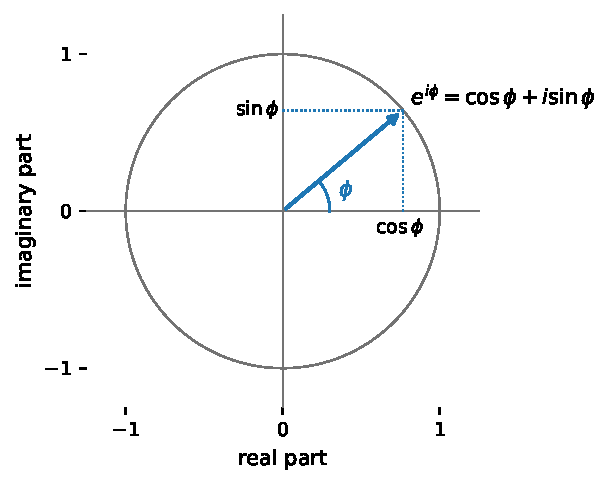
\includegraphics[width=0.36\textwidth]{unit_circle}
\caption{A complex number of magnitude one, $e^{i\phi}$, is a point on the unit circle at angle $\phi$.}
\label{fig:circle}
\end{figure}

\section{The state of a qubit}

The two classical values are the two unit vectors of the plane, and a qubit state is any unit-length combination of them:
\begin{equation}
\ket{0} = \begin{pmatrix}1\\0\end{pmatrix},\qquad
\ket{1} = \begin{pmatrix}0\\1\end{pmatrix},\qquad
\ket{\psi} = \alpha\ket{0} + \beta\ket{1} = \begin{pmatrix}\alpha\\\beta\end{pmatrix},\qquad
|\alpha|^2 + |\beta|^2 = 1 .
\label{eq:state}
\end{equation}
The complex numbers $\alpha$ and $\beta$ are the \emph{amplitudes}. The rule that connects them to what a measurement returns is the \emph{Born rule}:
\begin{equation}
P(0) = |\alpha|^2, \qquad P(1) = |\beta|^2 .
\label{eq:born}
\end{equation}
The normalization condition in Eq.~\eqref{eq:state} is exactly the statement that these two probabilities sum to one.

Because amplitudes are complex rather than positive, two different states can have identical probabilities. The notebook's first example is the pair
\begin{equation}
\ket{+} = \frac{1}{\sqrt2}\begin{pmatrix}1\\1\end{pmatrix}, \qquad
\ket{-} = \frac{1}{\sqrt2}\begin{pmatrix}1\\-1\end{pmatrix},
\label{eq:plusminus}
\end{equation}
both of which give $P(0) = P(1) = 1/2$. Sections~\ref{sec:phases} and~\ref{sec:interference} show that the sign is nevertheless real and measurable. Qiskit's \code{Statevector} stores the two amplitudes, and \code{sample\_counts(shots)} draws from the probabilities of Eq.~\eqref{eq:born}, which is the same thing as running a circuit that prepares the state and measures it. Sampling $\ket{+}$ 1000 times gave 502 zeros and 498 ones (Figure~\ref{fig:plus}). The notebook's exercise asks for a state with $P(0) = 0.8$; by Eq.~\eqref{eq:born} any $\alpha = \sqrt{0.8} \approx 0.894$ and $|\beta| = \sqrt{0.2} \approx 0.447$ will do, with any relative phase between $\alpha$ and $\beta$. The three vectors $(0.894, 0.447)$, $(0.894, -0.447)$, and $(0.894, 0.447i)$ all pass the Checkpoint, and all three are different states; a measurement in the $\ket{0},\ket{1}$ basis cannot tell them apart, but a measurement in another basis can, which is the subject of Section~\ref{sec:phases}.

\begin{figure}[h]
\centering
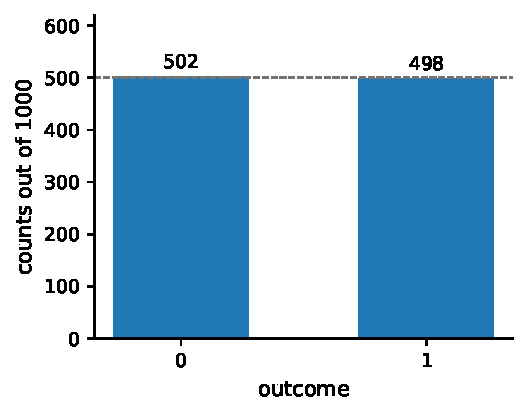
\includegraphics[width=0.42\textwidth]{plus_sampled}
\caption{1000 samples of $\ket{+}$ from \code{Statevector.sample\_counts}: the Born rule turned into counts.}
\label{fig:plus}
\end{figure}

\section{Dirac notation}

The column vector $\ket{\psi}$ is a \emph{ket}. The \emph{bra} $\bra{\psi}$ is the same vector written as a row with every entry conjugated,
\begin{equation}
\bra{\psi} = \begin{pmatrix}\bar\alpha & \bar\beta\end{pmatrix} .
\end{equation}
A bra followed by a ket is a row times a column, a single number called the \emph{inner product}:
\begin{equation}
\braket{\phi|\psi} = \sum_i \bar\phi_i\,\psi_i .
\label{eq:inner}
\end{equation}
In numpy, \code{np.vdot(phi, psi)} conjugates its first argument and so computes exactly this; in Qiskit, \code{phi.inner(psi)} does the same for two \code{Statevector}s. Three consequences of Eq.~\eqref{eq:inner} carry the day.
\begin{itemize}
\item $\braket{\psi|\psi} = \sum_i |\psi_i|^2 = 1$ for every normalized state.
\item $\braket{0|1} = 0$. Two states with zero inner product are \emph{orthogonal}, and orthogonal states are the ones a measurement can tell apart with certainty. The pair $\ket{+}$, $\ket{-}$ is also orthogonal: $\braket{+|-} = \tfrac12(1 - 1) = 0$.
\item $\braket{0|\psi} = \alpha$, so the Born rule reads $P(0) = |\braket{0|\psi}|^2$: the probability of an outcome is the squared inner product with that outcome's basis vector. This form generalizes to every measurement in the bootcamp.
\end{itemize}

A ket followed by a bra is a column times a row, a $2\times2$ matrix called the \emph{outer product}. The two that matter are the \emph{projectors} onto the basis states,
\begin{equation}
P_0 = \ket{0}\bra{0} = \begin{pmatrix}1&0\\0&0\end{pmatrix},\qquad P_1 = \ket{1}\bra{1} = \begin{pmatrix}0&0\\0&1\end{pmatrix},\qquad P_0 + P_1 = I,\quad P_x^2 = P_x .
\label{eq:projectors}
\end{equation}
The Born rule can be written with them as $P(x) = \braket{\psi|P_x|\psi}$, and $P_0 + P_1 = I$ is then the statement that the probabilities sum to $\braket{\psi|\psi} = 1$. The projector also says what is left after the measurement: the state collapses to $P_x\ket{\psi}/\sqrt{P(x)}$, which for $x = 0$ is $\alpha\ket{0}/|\alpha| = \ket{0}$ up to a phase. Measuring again applies $P_0$ once more, and $P_0^2 = P_0$ is why the second reading agrees with the first.

Table~\ref{tab:inner} lists the values Eq.~\eqref{eq:inner} predicts for the pairs in the notebook, and what \code{Statevector.inner} returns.

\begin{table}[h]
\centering
\small
\begin{tabular}{@{}lll@{}}
\toprule
& from Eq.~\eqref{eq:inner} & \code{Statevector.inner} \\
\midrule
$\braket{0|1}$ & $0$ & $0$ \\
$\braket{0|+}$ & $1/\sqrt2$ & $0.7071$ \\
$|\braket{0|+}|^2$ & $1/2$ & $0.5000$ \\
$\braket{+|-}$ & $0$ & $0$ \\
\bottomrule
\end{tabular}
\caption{Inner products of the basis states, predicted and computed.}
\label{tab:inner}
\end{table}

\begin{table}[h]
\centering
\small
\begin{tabular}{@{}llll@{}}
\toprule
State & Column vector & $P(0)$ & \code{Statevector.from\_label} \\
\midrule
$\ket{0}$ & $(1, 0)$ & 1 & \code{"0"} \\
$\ket{1}$ & $(0, 1)$ & 0 & \code{"1"} \\
$\ket{+}$ & $(1, 1)/\sqrt2$ & 1/2 & \code{"+"} \\
$\ket{-}$ & $(1, -1)/\sqrt2$ & 1/2 & \code{"-"} \\
$\ket{{+}i}$ & $(1, i)/\sqrt2$ & 1/2 & \code{"r"} \\
$\ket{{-}i}$ & $(1, -i)/\sqrt2$ & 1/2 & \code{"l"} \\
\bottomrule
\end{tabular}
\caption{The six states that sit on the axes of the Bloch sphere (Section~\ref{sec:bloch}), and the labels Qiskit uses for them.}
\label{tab:states}
\end{table}

\section{Global phase and relative phase}
\label{sec:phases}

Multiply an entire state by a magnitude-one number $e^{i\gamma}$. Every probability is unchanged, because $|e^{i\gamma}\psi_i|^2 = |\psi_i|^2$, and the same is true after any gate $U$, because gates are linear: $U(e^{i\gamma}\ket{\psi}) = e^{i\gamma}U\ket{\psi}$. No experiment can detect a \emph{global phase}, so $\ket{\psi}$ and $e^{i\gamma}\ket{\psi}$ are the same physical state. Qiskit's \code{Statevector.equiv} compares states up to exactly this freedom.

A phase between the two amplitudes is different. The states in Eq.~\eqref{eq:plusminus} differ by the sign of $\beta$ alone, a \emph{relative phase} of $e^{i\pi} = -1$, and they are orthogonal, which is as different as two states can be. A measurement in the $\ket{0}, \ket{1}$ basis cannot see the difference: both give 50/50. Applying $H$ first (Section~\ref{sec:gates}) maps $\ket{+}$ to $\ket{0}$ and $\ket{-}$ to $\ket{1}$, after which the measurement separates them perfectly (Figure~\ref{fig:bases}). Choosing what to apply before measuring is choosing the \emph{basis} of the measurement; Day~4 returns to this.

\begin{figure}[h]
\centering
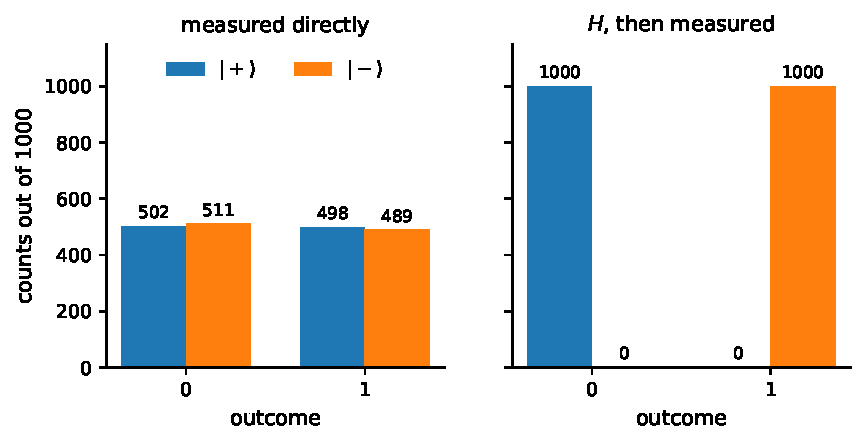
\includegraphics[width=0.72\textwidth]{plus_minus_bases}
\caption{$\ket{+}$ and $\ket{-}$ on the simulator, 1000 shots each. Measured directly (left) they gave 502/498 and 511/489. After an $H$ (right) $\ket{+}$ gave 1000 zeros and $\ket{-}$ gave 1000 ones: the relative sign has become a definite outcome.}
\label{fig:bases}
\end{figure}

\section{The Bloch sphere}
\label{sec:bloch}

Two complex amplitudes are four real numbers. Normalization removes one and the invisible global phase removes another, leaving two. Use the global phase to make $\alpha$ real and non-negative; then $\alpha = \cos\frac\theta2$ for a unique $\theta \in [0, \pi]$, normalization forces $|\beta| = \sin\frac\theta2$, and the remaining freedom in $\beta$ is its angle $\phi$:
\begin{equation}
\ket{\psi} = \cos\tfrac{\theta}{2}\,\ket{0} + e^{i\phi}\sin\tfrac{\theta}{2}\,\ket{1}, \qquad 0 \le \theta \le \pi,\quad 0 \le \phi < 2\pi .
\label{eq:bloch}
\end{equation}
A pair of angles like this is a point on a sphere (Figure~\ref{fig:bloch}). The north pole $\theta = 0$ is $\ket{0}$, the south pole $\theta = \pi$ is $\ket{1}$, and the equator $\theta = \pi/2$ holds every 50/50 state: $\ket{+}$ at $\phi = 0$, $\ket{{+}i}$ at $\phi = \pi/2$, $\ket{-}$ at $\phi = \pi$, $\ket{{-}i}$ at $\phi = 3\pi/2$. Orthogonal states sit at antipodal points. The half-angle $\theta/2$ in Eq.~\eqref{eq:bloch} is what makes orthogonal states land opposite each other rather than at right angles.

The sphere is a one-qubit picture and stops there. The same count for $n$ qubits gives $2\cdot2^n$ real numbers, less one for normalization and one for the global phase, so two qubits already need six parameters and no surface in three dimensions can hold them. What survives to any number of qubits is the coordinate version of the sphere below: each qubit's expectation values $(\braket X, \braket Y, \braket Z)$ can always be measured, and for an entangled pair they are shorter than unit length, a fact Day~4 uses to detect entanglement.

\begin{figure}[h]
\centering
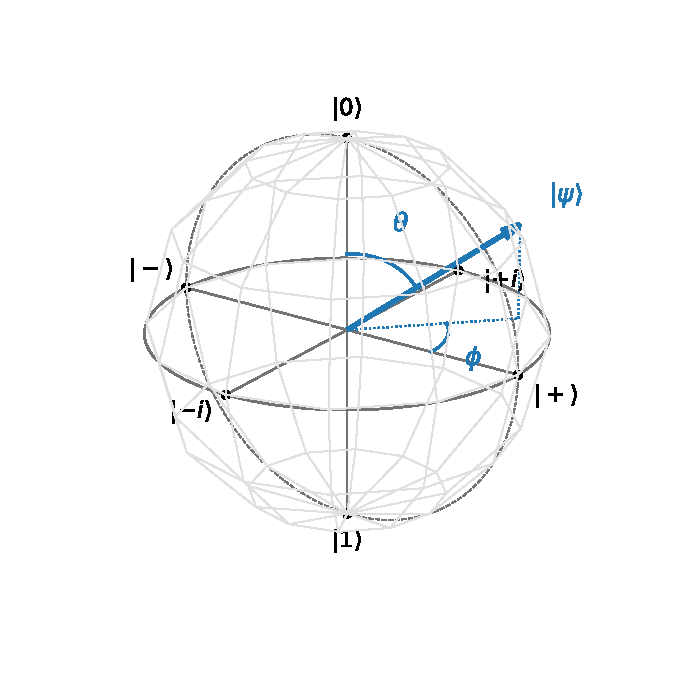
\includegraphics[width=0.58\textwidth]{bloch_sphere}
\caption{The Bloch sphere. The six axis states of Table~\ref{tab:states} sit on the axes; the state of Eq.~\eqref{eq:bloch} with $\theta = \pi/3$, $\phi = \pi/4$ is the blue arrow.}
\label{fig:bloch}
\end{figure}

The sphere is more than a picture. Its Cartesian coordinates are three quantities a measurement can estimate, the \emph{expectation values} of the Pauli matrices of Section~\ref{sec:gates}. For $Z$, which has $\ket{0}$ and $\ket{1}$ as eigenvectors with eigenvalues $\pm1$,
\begin{equation}
\braket{Z} = P(0) - P(1) = \cos^2\tfrac\theta2 - \sin^2\tfrac\theta2 = \cos\theta ,
\end{equation}
and a short calculation gives the other two. Multiplying out $\bra{\psi}X\ket{\psi}$ with the matrix of Section~\ref{sec:gates} gives $\bar\alpha\beta + \bar\beta\alpha = 2\,\mathrm{Re}(\bar\alpha\beta)$, and with $\alpha = \cos\frac\theta2$, $\beta = e^{i\phi}\sin\frac\theta2$ this is $2\cos\frac\theta2\sin\frac\theta2\cos\phi = \sin\theta\cos\phi$ by the double-angle formula; the same steps for $Y$ replace the real part by the imaginary part and give $\sin\theta\sin\phi$. Together:
\begin{equation}
\big(\braket{X}, \braket{Y}, \braket{Z}\big) = \big(\sin\theta\cos\phi,\ \sin\theta\sin\phi,\ \cos\theta\big) .
\label{eq:blochvec}
\end{equation}
This is the unit vector at polar angle $\theta$ and azimuth $\phi$. The notebook's \code{bloch\_vector} function computes it with \code{state.expectation\_value(Pauli("X"))} and checks Eq.~\eqref{eq:blochvec} numerically. For the state with $\theta = \pi/3$, $\phi = \pi/4$ that the notebook draws (Figure~\ref{fig:blochpsi}), the formula gives $(0.612,\ 0.612,\ 0.500)$ and the three expectation values from Qiskit are $(0.612,\ 0.612,\ 0.500)$.

\begin{figure}[h]
\centering
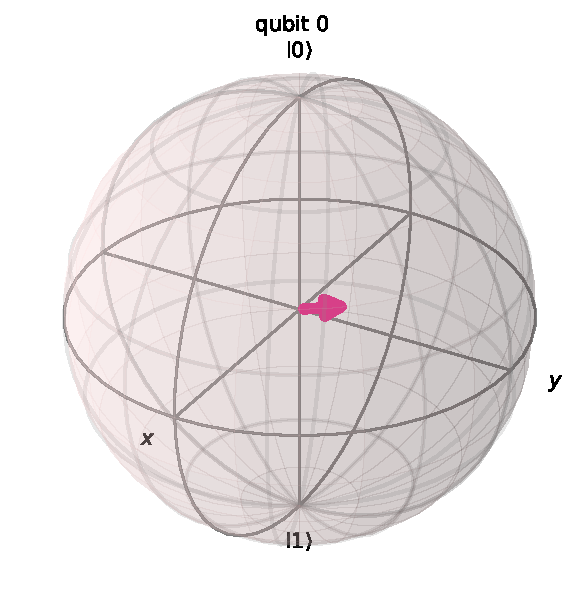
\includegraphics[width=0.36\textwidth]{bloch_psi_qiskit}
\caption{Qiskit's \code{plot\_bloch\_multivector} of the state with $\theta = \pi/3$, $\phi = \pi/4$.}
\label{fig:blochpsi}
\end{figure}

\section{Gates are unitary matrices}
\label{sec:gates}

A gate on one qubit is a $2\times2$ matrix $U$ acting by multiplication, $\ket{\psi} \mapsto U\ket{\psi}$. The output must still be a valid state, so $U$ must preserve the norm of every input. Writing the output's norm as $\bra{\psi}U^\dagger U\ket{\psi}$, with $U^\dagger$ the conjugate transpose, this holds for all $\ket{\psi}$ exactly when
\begin{equation}
U^\dagger U = I .
\label{eq:unitary}
\end{equation}
A matrix satisfying Eq.~\eqref{eq:unitary} is \emph{unitary}. It always has an inverse, namely $U^\dagger$ itself, so every quantum gate is reversible: apply $U^\dagger$ and the input is back. Two more facts follow directly. A unitary preserves every inner product, $\braket{U\phi|U\psi} = \bra{\phi}U^\dagger U\ket{\psi} = \braket{\phi|\psi}$, so orthogonal states stay orthogonal and a gate can never make two distinguishable states harder to tell apart. And every eigenvalue $\lambda$ of a unitary has $|\lambda| = 1$, because $U\ket{v} = \lambda\ket{v}$ and $\|U v\| = \|v\|$ force $|\lambda|\,\|v\| = \|v\|$; the eigenvalues of $X$, $Y$, $Z$, and $H$ are all $\pm1$. Checking Eq.~\eqref{eq:unitary} for $H$ takes one line: $H$ is real and symmetric, so $H^\dagger = H$, and $H^2 = \tfrac12\begin{pmatrix}2&0\\0&2\end{pmatrix} = I$. This is the quantum counterpart of the observation on Day~1 that NOT can be undone but AND cannot. The three gates of the week are
\begin{equation}
X = \begin{pmatrix}0&1\\1&0\end{pmatrix},\qquad
Z = \begin{pmatrix}1&0\\0&-1\end{pmatrix},\qquad
H = \frac{1}{\sqrt2}\begin{pmatrix}1&1\\1&-1\end{pmatrix},
\label{eq:xzh}
\end{equation}
together with the third Pauli matrix $Y = \begin{pmatrix}0&-i\\i&0\end{pmatrix} = iXZ$. Table~\ref{tab:gates} lists what they do to the basis states; each row is one matrix-vector product. On the Bloch sphere, $X$, $Y$, and $Z$ are half-turns about the $x$, $y$, and $z$ axes, and $H$ is a half-turn about the axis halfway between $x$ and $z$, which is why it swaps the poles with $\ket{\pm}$.

\begin{table}[h]
\centering
\small
\begin{tabular}{@{}lllll@{}}
\toprule
Gate & On $\ket{0}$ & On $\ket{1}$ & On $\ket{+}$ & Bloch sphere \\
\midrule
$X$ & $\ket{1}$ & $\ket{0}$ & $\ket{+}$ & half-turn about $x$ \\
$Y$ & $i\ket{1}$ & $-i\ket{0}$ & $-i\ket{-}$ & half-turn about $y$ \\
$Z$ & $\ket{0}$ & $-\ket{1}$ & $\ket{-}$ & half-turn about $z$ \\
$H$ & $\ket{+}$ & $\ket{-}$ & $\ket{0}$ & half-turn about $(x+z)/\sqrt2$ \\
\bottomrule
\end{tabular}
\caption{Actions of the single-qubit gates used this week. $X$ swaps amplitudes, $Z$ flips the relative sign, $H$ moves between the $\{\ket0,\ket1\}$ and $\{\ket+,\ket-\}$ bases.}
\label{tab:gates}
\end{table}

In Qiskit, \code{Operator(M)} wraps a matrix and \code{state.evolve(Operator(M))} applies it. A whole circuit is itself one matrix, the product of its gates, and \code{Operator(qc)} computes it:
\begin{lstlisting}
qc = QuantumCircuit(1)
qc.h(0)
Operator(qc).data          # the 2x2 matrix H
sv0.evolve(Operator(H))    # H|0> = |+>
\end{lstlisting}

\section{Interference}
\label{sec:interference}

Apply $H$ twice to $\ket{0}$. The amplitude to end in $\ket{1}$ is the $(1,0)$ entry of the product $HH$, which the rule for matrix multiplication writes as a sum over the intermediate state $k$:
\begin{equation}
\braket{1|HH|0} = \sum_{k\in\{0,1\}} H_{1k}H_{k0}
= \underbrace{\tfrac{1}{\sqrt2}\cdot\tfrac{1}{\sqrt2}}_{\text{via }\ket{0}}
+ \underbrace{\big(-\tfrac{1}{\sqrt2}\big)\cdot\tfrac{1}{\sqrt2}}_{\text{via }\ket{1}}
= \tfrac12 - \tfrac12 = 0 .
\label{eq:paths}
\end{equation}
Each path on its own would contribute probability $1/4$. Together they contribute nothing, because the path through $\ket{1}$ picks up the minus sign in the lower-right entry of $H$. Probabilities are non-negative and can only add; amplitudes carry signs and can cancel. This is \emph{interference}, and it is the mechanism every quantum algorithm relies on: arrange the phases so that paths to wrong answers cancel and paths to the right answer reinforce. In matrix language the same statement is $HH = I$. The path picture is nothing more than the rule for multiplying matrices, and it holds for any sequence of gates: the amplitude to go from $\ket{a}$ to $\ket{b}$ through gates $U_1, U_2, \ldots, U_L$ is a sum over every choice of intermediate basis state, each term the product of one matrix entry per gate. For one qubit and $L$ gates there are $2^{L-1}$ such paths; for $n$ qubits there are $(2^n)^{L-1}$, and a quantum computer adds them all at once.

Insert a $Z$ between the two Hadamards. $Z$ multiplies the $\ket{1}$ component by $-1$, so the second path in Eq.~\eqref{eq:paths} changes sign and the two paths now add to one: $\braket{1|HZH|0} = 1$. The qubit ends in $\ket{1}$ every time, which is the statement
\begin{equation}
HZH = X .
\label{eq:hzh}
\end{equation}
Figure~\ref{fig:paths} draws both cases. Multiplying out the matrices in Eq.~\eqref{eq:xzh} confirms Eq.~\eqref{eq:hzh}, and the notebook's Checkpoint does so numerically. The notebook's runs agree: 1000 shots after $HH$ all read 0, and 1000 shots after $HZH$ all read 1.

\begin{figure}[h]
\centering
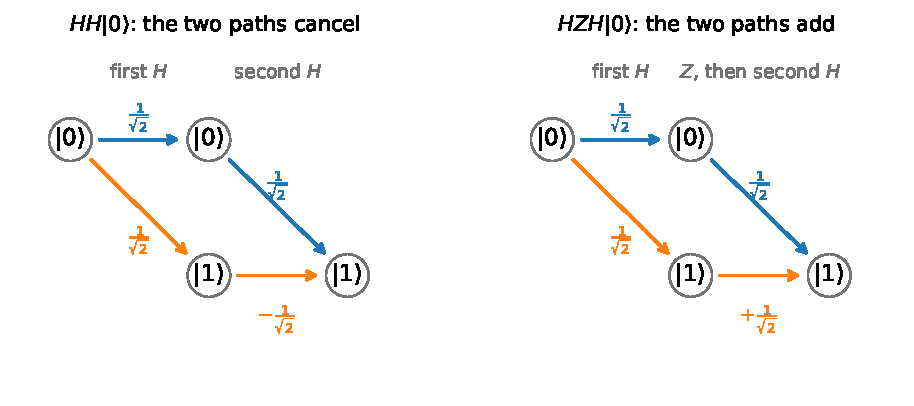
\includegraphics[width=0.95\textwidth]{interference_paths}
\caption{The two paths from $\ket{0}$ to $\ket{1}$. Left: through $HH$ the path amplitudes are $+\tfrac12$ and $-\tfrac12$ and cancel. Right: a $Z$ between the Hadamards flips the sign of the lower path, so its second leg carries $(-1)(-\tfrac{1}{\sqrt2}) = +\tfrac{1}{\sqrt2}$ and the amplitudes add to 1.}
\label{fig:paths}
\end{figure}

\section{Simulator versus hardware}
\label{sec:hardware}

Notebook section 9 sends the four circuits of Section~\ref{sec:phases} to a quantum processor: $\ket{+}$ and $\ket{-}$ measured directly, then measured after an $H$. On the simulator the four give 487/513, 505/495, 1000/0, and 0/1000: the direct pair is a fair coin and the after-$H$ pair is certain, because $H\ket{+} = \ket{0}$ is an identity of linear algebra. The recorded run on \code{ibm\_kingston}, 1000 shots per circuit on physical qubit~0, gave 321/679, 333/667, 459/541, and 168/832 (Figure~\ref{fig:hardware}). Nothing about that is a few percent in the wrong bin, and the reason is worth working out, because it is the first real device error in the bootcamp.

Start with the two after-$H$ circuits. Before submitting, the transpiler simplified them: $H$ then $H$ cancels to nothing, so the third circuit is a bare measurement of $\ket{0}$, and $H$, $Z$, $H$ is $X$ by Eq.~\eqref{eq:hzh}, so the fourth is an $X$ gate followed by a measurement. Those two circuits are therefore a readout test: prepare $\ket{0}$ and $\ket{1}$, and see what comes back. On that qubit that day, a prepared $\ket{0}$ was read as 1 in 54\% of shots and a prepared $\ket{1}$ as 0 in 17\%. Collect the four rates into a matrix whose columns are the prepared state and whose rows are the reported one,
\begin{equation}
M = \begin{pmatrix}0.459 & 0.168\\ 0.541 & 0.832\end{pmatrix},
\label{eq:readout}
\end{equation}
and the direct measurements follow. A fair coin seen through this readout is reported as $\tfrac12(0.459 + 0.168) = 31\%$ zeros and $69\%$ ones; the two direct circuits gave 32\% and 33\% zeros. Nothing was wrong with $\ket{+}$ or $\ket{-}$, and the relative sign was as invisible to a direct measurement as Section~\ref{sec:phases} says; the measurement itself was misreporting, far outside the 1.9\% readout error in the qubit's calibration table. Solving $M\vec p_{\rm true} = \vec p_{\rm reported}$ for the direct runs returns $P(0) = 0.53$ and $0.57$, back near the fair coin, which is the idea behind the readout mitigation of Day~5. The same qubit produced the 70/30 random bit of Day~1 forty minutes earlier, for the same reason.

\begin{figure}[h]
\centering
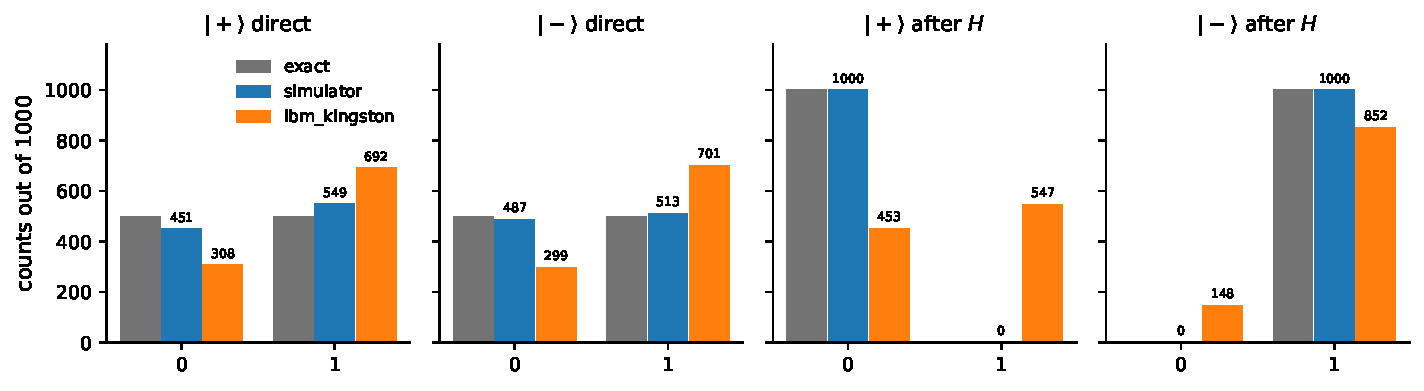
\includegraphics[width=0.98\textwidth]{hardware_four}
\caption{The four circuits of notebook section 9 on the simulator and on \code{ibm\_kingston}, 1000 shots each. The two right-hand panels are, after transpilation, a measurement of $\ket{0}$ and of $\ket{1}$, and read off the readout matrix of Eq.~\eqref{eq:readout}.}
\label{fig:hardware}
\end{figure}

\section{Summary}

\begin{itemize}
\item A complex number is a magnitude and an angle, $z = re^{i\phi}$. Magnitude-one numbers are pure angles, and their angles add under multiplication.
\item A qubit is a normalized vector $\alpha\ket0 + \beta\ket1$, Eq.~\eqref{eq:state}. The Born rule, Eq.~\eqref{eq:born}, turns amplitudes into probabilities.
\item Bras are conjugated rows, kets are columns, and $\braket{\phi|\psi}$ is their inner product. Orthogonal states are perfectly distinguishable, and $P(x) = |\braket{x|\psi}|^2$.
\item A global phase is invisible. A relative phase is a different state, visible after a change of basis (Figure~\ref{fig:bases}).
\item Every qubit state is a point $(\theta, \phi)$ on the Bloch sphere, Eq.~\eqref{eq:bloch}, whose coordinates are the expectation values $(\braket X, \braket Y, \braket Z)$, Eq.~\eqref{eq:blochvec}.
\item Gates are unitary matrices, $U^\dagger U = I$, hence reversible. $X$ swaps amplitudes, $Z$ flips a sign, $H$ changes basis.
\item Amplitudes add along paths and can cancel: $HH = I$ by Eq.~\eqref{eq:paths}, and $HZH = X$ when a sign flip turns cancellation into reinforcement.
\end{itemize}

\begin{thebibliography}{9}
\bibitem{watrous} J.~Watrous, \emph{Basics of Quantum Information}, lesson 1, Single systems. IBM Quantum Learning. \url{https://quantum.cloud.ibm.com/learning/en/courses/basics-of-quantum-information/single-systems/introduction}
\bibitem{nielsen} M.~A. Nielsen and I.~L. Chuang, \emph{Quantum Computation and Quantum Information}, 10th anniversary ed. (Cambridge University Press, 2010), sections 1.2 and 1.3.
\bibitem{mermin} N.~D. Mermin, \emph{Quantum Computer Science: An Introduction} (Cambridge University Press, 2007), chapter~1.
\bibitem{statevector} Qiskit API reference, \code{qiskit.quantum\_info.Statevector}. \url{https://quantum.cloud.ibm.com/docs/en/api/qiskit/qiskit.quantum_info.Statevector}
\bibitem{operator} Qiskit API reference, \code{qiskit.quantum\_info.Operator}. \url{https://quantum.cloud.ibm.com/docs/en/api/qiskit/qiskit.quantum_info.Operator}
\bibitem{bloch} F.~Bloch, ``Nuclear induction,'' Phys. Rev. \textbf{70}, 460 (1946), whose magnetization vector is the origin of the picture; the sphere itself is older, as Poincar\'e's sphere for polarization (1892).
\end{thebibliography}

\end{document}
